\chapter{Despliegue en la nube}

Hemos elegido Amazon Web Service como servicio de computación en la nube por el gran impacto que está teniendo en el mundo laboral, mayor que sus competidores directos como son Azure y Google Cloud.

Otro factor que juega a favor de AWS con respecto a sus competidores es que a la hora de desplegar una aplicación en la nube la experiencia de usuario resulta mucho mas intuitiva que la de sus competidores. También ofrece un buen soporte, donde en cualquier momento te resuelven las posibles dudas a la hora de desplegar la aplicación.

Por último y como factor de bastante importancia para aquellos pequeños emprendedores que quiera empezar a desarrollar sus ideas, es el bajo coste que supone tener una aplicación desplegada en la nube de Amazon. Por el momento, el primer año de tu cuenta en AWS es gratuita, restringida a ciertas limitaciones.


Hoy en día, Amazon Web Services proporciona una plataforma de infraestructura escalable, de confianza y de bajo costo en la nube que impulsa cientos de miles de negocios de 190 países de todo el mundo. Con centros de datos en Estados Unidos, Europa, Brasil, Singapur, Japón y Australia. Por ejemplo:

\begin{enumerate}
     \item \textbf{Amazon.com: } Es el minorista online más grande del mundo. En 2011, Amazon.com pasó de utilizar el backup en cinta a usar Amazon S3 en la cloud para realizar copias de seguridad de la mayoría de las bases de datos de Oracle de las que se encarga. Mediante el uso de AWS, Amazon.com logró eliminar el software de backup y experimentó una mejora de desempeño 12 veces mayor, de forma que pudo reducir el tiempo de restablecimiento de 15 a 2,5 horas aproximadamente en situaciones seleccionadas.
    \item \textbf{Netflix: } El referente de la televisión en streaming usa AWS para proporcionar miles de millones de horas de vídeo casa mes a sus mas de 60 millones de suscriptores. Así puede hacer uso de miles de servidores y terabites de almacenamiento en cuestión de minutos para que sus usuarios puedan ver series y películas desde cualquier parte del mundo en sus tabletas o teléfonos móviles.
    \item \textbf{Dropbox: } El famoso y conocido servicio de alojamiento de archivos multiplataforma en la nube utiliza hasta el momento AWS como repositorio para almacenar todos los archivos que los usuarios de Dropbox suben a la red.
    \item \textbf{FC Barcelona: }Su sitio web, que aloja más de 6 000 páginas y 12.000 fotos digitales, también usa AWS para su mantenimiento.
    \item \textbf{Harvard Medical School} Desarrolla nuevos modelos de pruebas de genomas en tiempo récord.
    \item \textbf{Mapfre: }Ahorró 1,3 millones de euros en infraestructura y redujo el desarrollo de semanas a días

\end{enumerate}

\section{Lanzar una instancia en AWS}

Antes de subir nuestra aplicación a producción debemos de crear una instancia en AWS. Estos son los pasos a tener en cuenta a la hora de crear una instancia en AWS:

\begin{itemize}
    \item \textbf{Paso1. Crear Key Pairs} Los \textit{Key Pairs} se utilizan para iniciar sesión de forma segura en los servicios de AWS. Crearemos un Key Pairs para acceder a nuestra instancia de EC2.
\begin{enumerate}
    \item Para crear nuevos pares de claves, de debe navegar hasta AWS Console y luego hacer clic en EC2.
    \begin{figure}[!h]
    \centering
    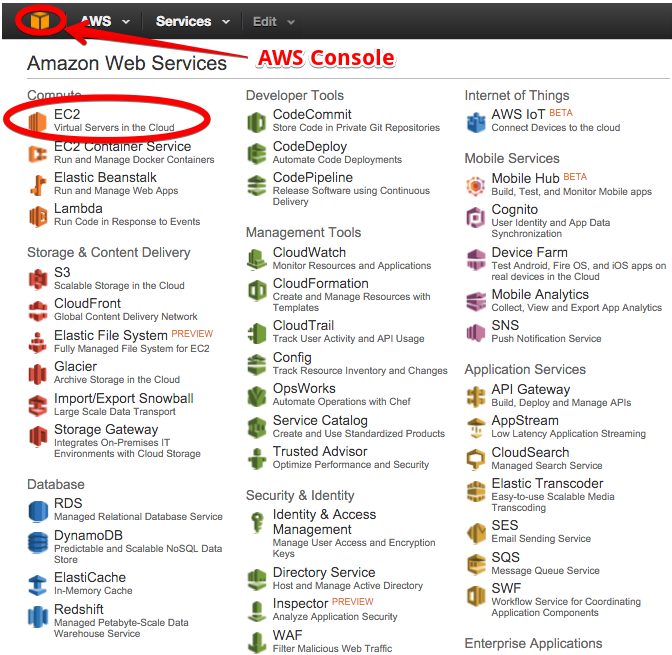
\includegraphics[width=90mm]{img/despliegue/paso1_1.png}
    \caption{Crear Key Pairs Paso 1}
    \end{figure}
    \item En el panel izquierdo, se debe hacer clic en Key Pairs, luego clic en Crear Key Pairs
     \begin{figure}[!h]
    \centering
    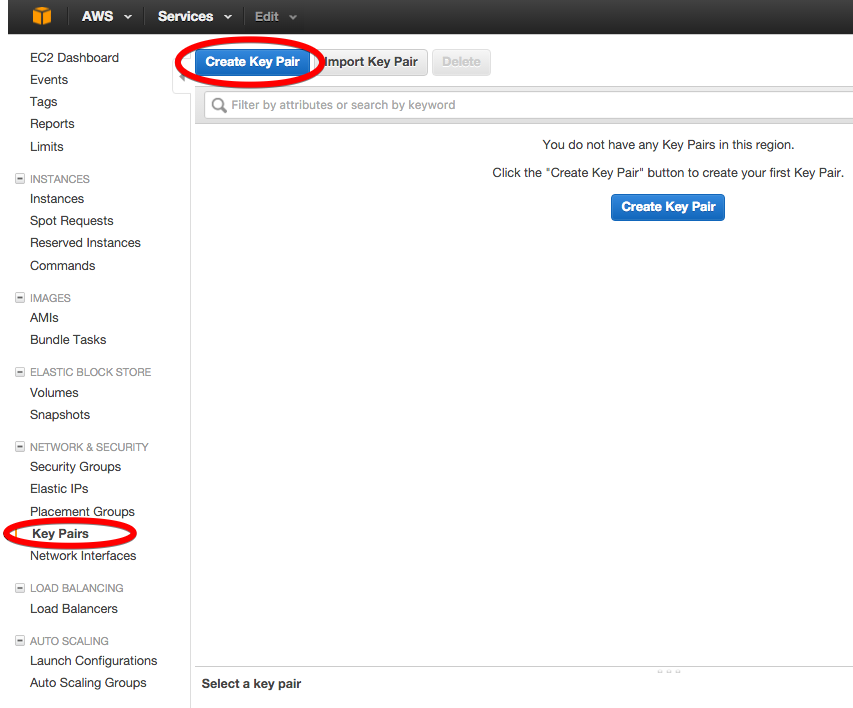
\includegraphics[width=90mm]{img/despliegue/paso1_2.png}
    \caption{Crear Key Pairs Paso 2}
    \end{figure}
    \item Se debe introducir un nombre para la clave, luego hacer clic en Crear Key Pairs. El Key Pairs se descargará automáticamente. Debe moverse esta clave a un directorio diferente.

    Importante: Se deberá cambiar los permisos de esta clave para que sean de solo lectura, con el siguiente código:
    \begin{lstlisting}
    chmod 400 youKeyName.pem
    \end{lstlisting}
\end{enumerate}
    \item \textbf{Paso 2. Lanza una instancia de EC2 con Bitnami} En este paso, lanzaremos una instancia de EC2 desde Amazon Machine Image (AMI). Con AMI se puede activar una instancia de EC2 que esté lista para el desarrollo sin demasiada configuración. Bitnami proporciona una imagen MEAN preconfigurada que usaremos para configurarlo rápidamente.

    \begin{enumerate}
    \item Primero se debe navegar a la consola de AWS y hacer clic en AWS Marketplace.
    \begin{figure}[!h]
    \centering
    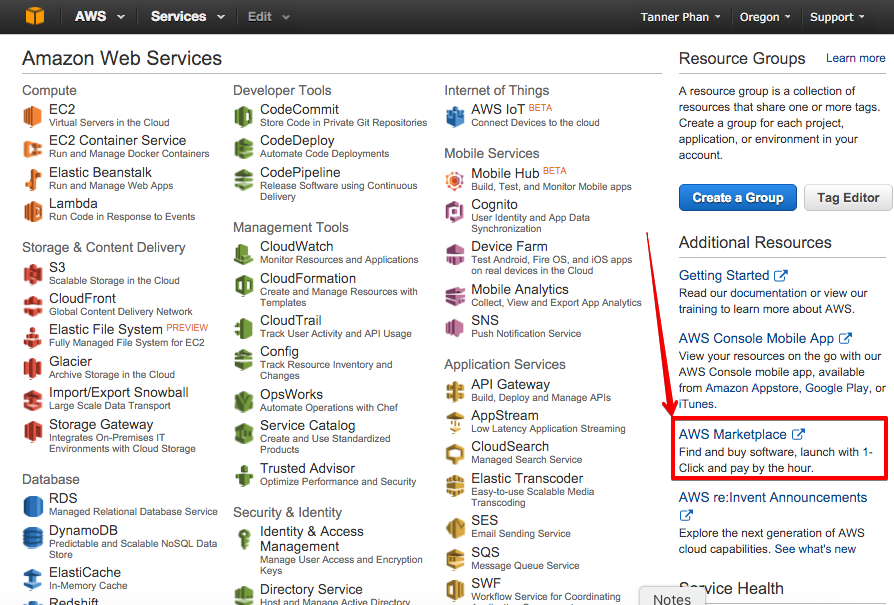
\includegraphics[width=90mm]{img/despliegue/paso2_1.png}
    \caption{Lanza una instancia Paso 1}
    \end{figure}
    \item Buscar MEAN powered en Bitnami, luego seleccione 64-bit AMI para continuar. Ver figura \ref{img:paso2}
    \begin{figure}[!h]
    \centering
    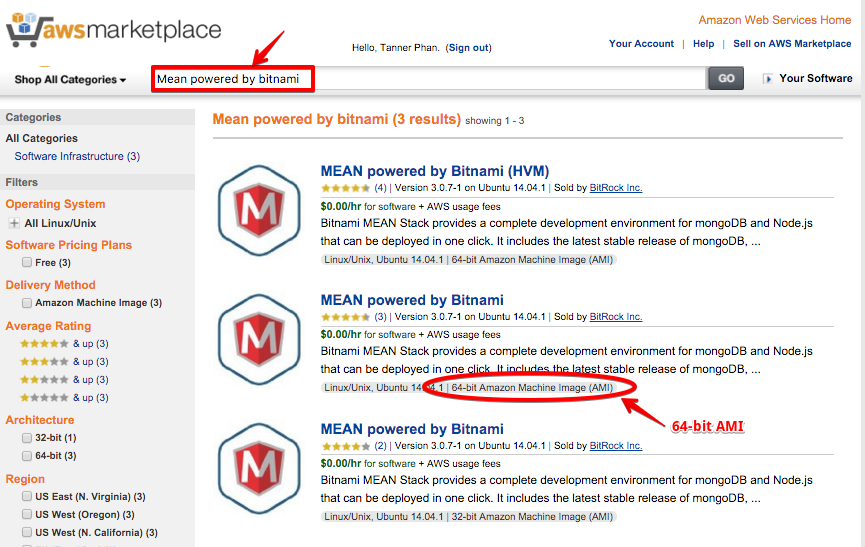
\includegraphics[width=90mm]{img/despliegue/paso2_2.png}
    \caption{Lanza una instancia Paso 2}
    \label{img:paso2}
    \end{figure}
    \item En el apartado \textit{Pricing Details} con el fin de obtener la mejor velocidad de entrega, seleccionar la región más cercana y luego hacer clic en Continuar. Ver figura \ref{img:paso3}
    \begin{figure}[!h]
    \centering
    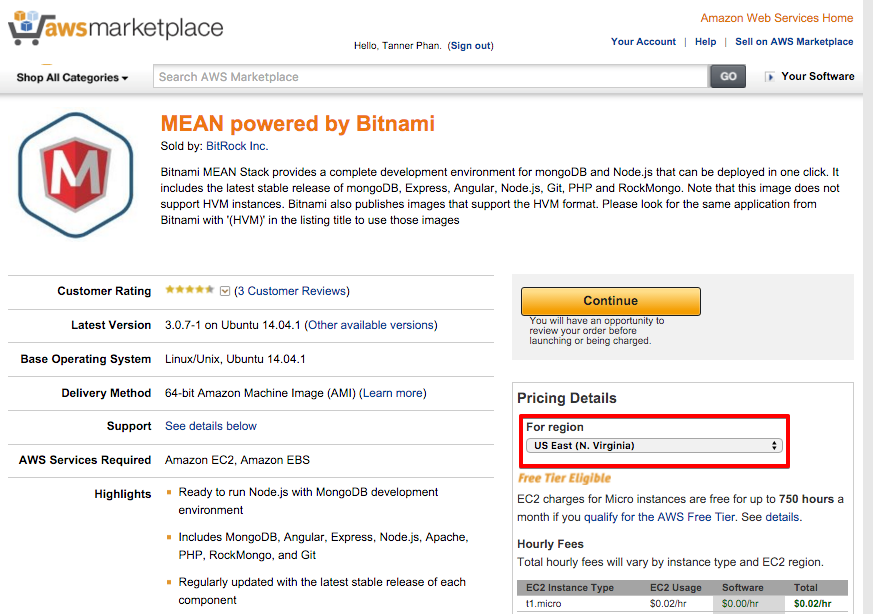
\includegraphics[width=90mm]{img/despliegue/paso2_3.png}
    \caption{Lanza una instancia Paso 3}
    \label{img:paso3}
    \end{figure}
    \item Para el grupo de seguridad, se ha de elegir 'Crear nuevo' según la configuración del vendedor.
    \item Asegurarse de tener los siguientes métodos de conexión:
    \begin{lstlisting}
     1.SSH, My IP
     2.HTTP, Anywhere
     3.HTTPS, Anywhere
    \end{lstlisting}
    \item Seleccionar la Key Pair que creaste en el paso 1.
    \item Finalmente, hacer clic en Iniciar para iniciar la instancia.
    \end{enumerate}
    \item \textbf{Paso 3. Conéctate a tu EC2} Para conectarse por SSH a la instancia, se necesitará la IP pública de su instancia y el Key Pair que creó.
    \begin{enumerate}
    \item Dentro de EC2, hacer clic en Instancias, seleccionar la instancia recién iniciada en el paso anterior y luego hacer clic en Conectar.
    \item Copiar el código que aparece marcado en rojo en la imagen \ref{img:paso4}.
    \begin{figure}[!h]
    \centering
    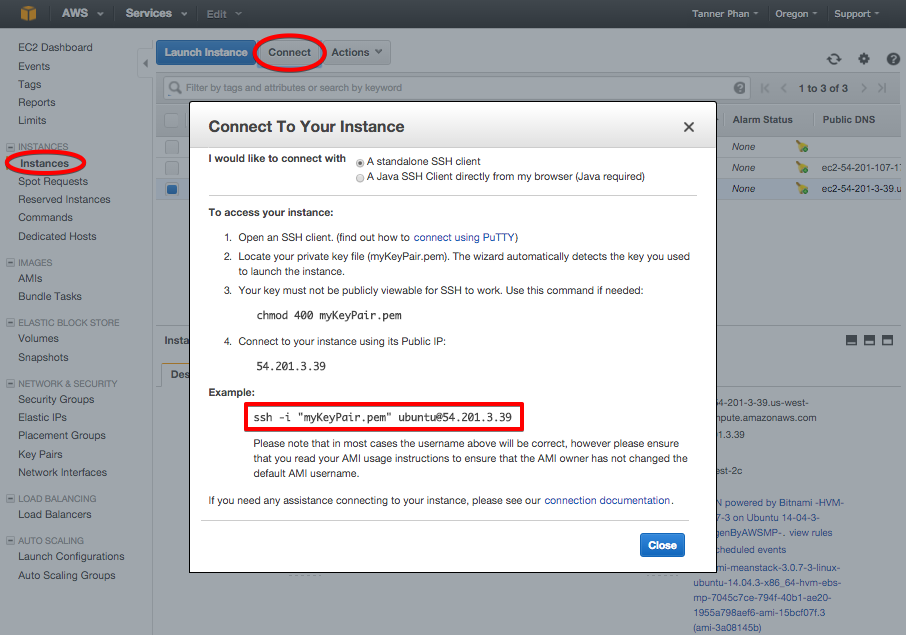
\includegraphics[width=90mm]{img/despliegue/paso3_2.png}
    \caption{Conéctate a tu EC2 Paso 2}
    \label{img:paso4}
    \end{figure}
    \item En su terminal, navegar hasta el directorio donde está guardado el par de claves, luego pegar el último paso del código.
    \begin{figure}[!h]
    \centering
    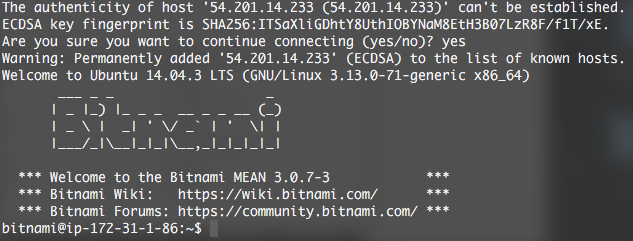
\includegraphics[width=90mm]{img/despliegue/paso3_3.png}
    \caption{Conéctate a tu EC2 Paso 3}
    \end{figure}
    \end{enumerate}

    \item \textbf{Paso 4. Conseguir un dominio} Una vez que ya tenemos la instancia creada y hemos sido capaces de conectarnos a ella por SSH, llega el momento de conseguir un dominio para que los usuarios se puedan conectar a la aplicación lo más fácilmente posible.
    El dominio que he utilizado es un dominio, proporcionado por el propio Amazon.

    \item \textbf{Paso 4. Obtener un certificado SSL gratis con AWS Certificate Manager}

    Un certificado SSL es un fichero informático generado por una entidad de servicios de certificación que asocia unos datos de identidad a una persona física, organismo o empresa, confirmando de esta manera su identidad digital en Internet. Necesitamos un certificado SSL para que los usuarios que accedan a nuestra página lo hagan de una forma segura por el protocolo HTTPS.

    Por otro lado tenemos Amazon CloudFront, es un servicio de red de entrega de contenido (CDN) global que proporciona datos, vídeos, aplicaciones y API de forma segura a sus espectadores con baja latencia y altas velocidades de transferencia.

    Para conseguir el certificado SSL en AWS se necesita seguir los siguientes pasos:

     \begin{enumerate}
        \item Ir a AWS \textit{manager certificate} desde la consola de Amazon web services y hacer click en \textit{get started}.
        \item A continuación te pedirá el dominio creado previamente y tendrás que hacer click en \textit{Review and request}.
        \item Una vez enviada la solicitud de certificado a la Autoridad certificadora, un email de confirmación será enviado a nuestra cuenta de correo vinculada con el dominio, es decir a admin@classcity.es.
        \item Una vez que recibimos un correo como el que aparece en la siguiente imagen, realizamos la confirmación del certificado haciendo click en el enlace que viene en el correo.
        \begin{figure}[!h]
        \centering
        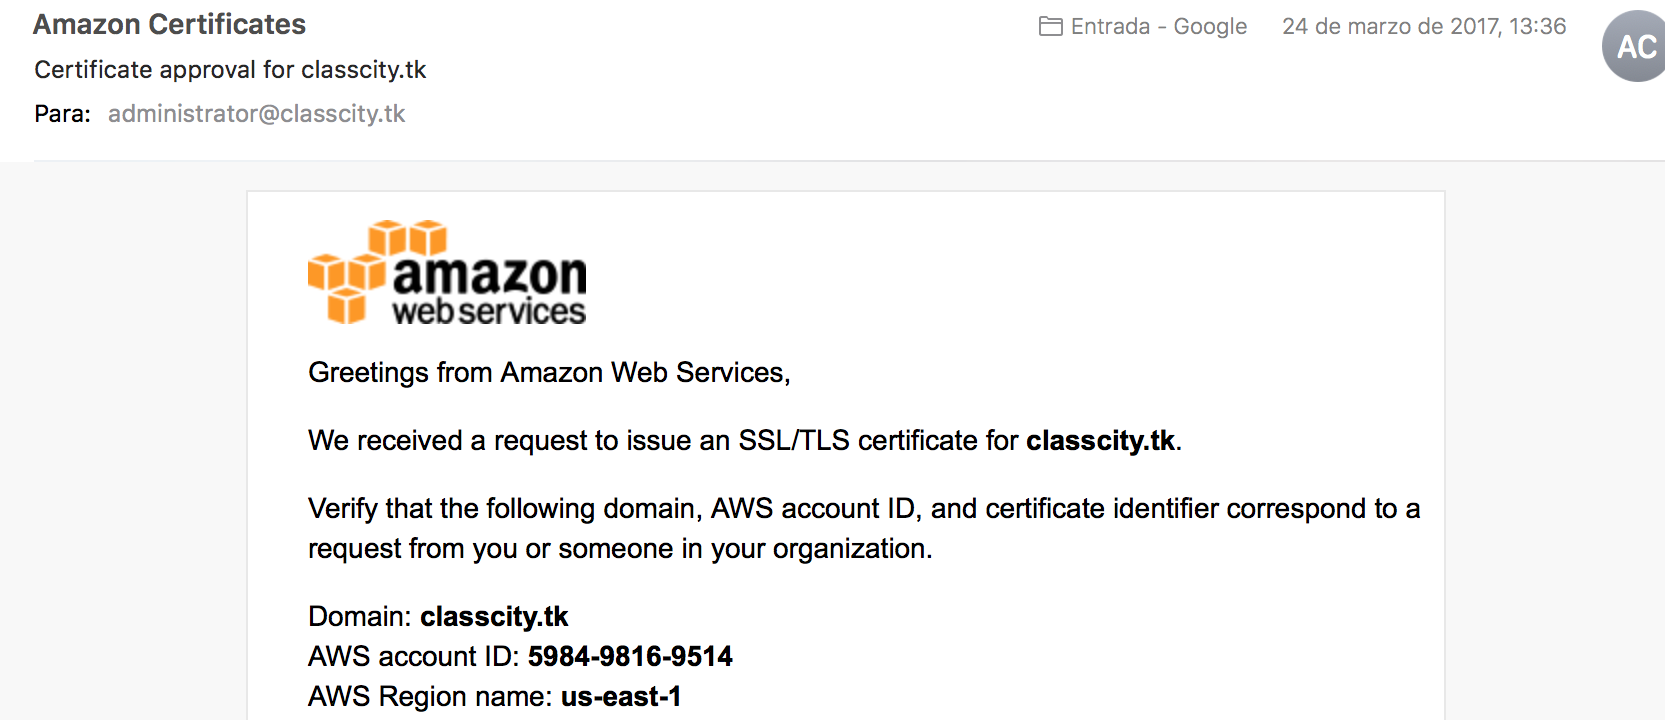
\includegraphics[width=80mm]{img/despliegue/ssl.png}
        \caption{Correo de confirmación}
        \end{figure}
    \end{enumerate}

    Si ahora vamos a nuestro dominio e introducimos antes el protocolo HTTPS, es decir en nuestro caso https://www.classcity.es, veremos que efectivamente accedemos a nuestra aplicacion de una forma segura. Ver figura \ref{img:dominio}

    \begin{figure}[!h]
    \centering
    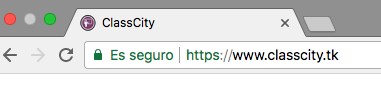
\includegraphics[width=80mm]{img/despliegue/https.png}
    \caption{SSL}
    \label{img:dominio}
    \end{figure}

\end{itemize}

\section{Lanzar una aplicación MEAN a producción} Una vez que dispongamos de una instancia, un dominio y un certificado SSL, tenemos todo listo para desplegar nuestra aplicación MEAN en producción. Para ello debemos seguir los siguientes pasos:

\begin{enumerate}
  \item Conectarnos desde nuestra terminal por SSH a nuestra máquina virtual de AWS
  \begin{lstlisting}
  sudo ssh -i /.ssh/keypair.pem root@ipinstance
  \end{lstlisting}
  \item Clonar en la máquina virtual de AWS nuestro repositorio git donde almacenemos la aplicación MEAN.
  \begin{lstlisting}
  rooti@ip sudo git clone https//github.com/RoboticsURJC-students/2016-tfg-Mario-Fernandez.git
  \end{lstlisting}
  \item Instalar dependencias de la aplicación web por parte del lado cliente.
  \begin{lstlisting}
  rooti@ip cd 2016-tfg-Mario-Fernandez
  rooti@ip /2016-tfg-Mario-Fernandez sudo npm install
  \end{lstlisting}
  \item Correr Angular con angular-ci.
  \begin{lstlisting}
  rooti@ip /2016-tfg-Mario-Fernandez sudo npm run build
  \end{lstlisting}
  \item Una nueva carpeta se crea al terminar el proceso ./dist, debemos copiarla entera en nuestra carpeta httdocs de apache.
  \begin{lstlisting}
  rooti@ip /2016-tfg-Mario-Fernandez sudo cp -r ./dist/* ../httdocs
  \end{lstlisting}
  \item Ahora deberíamos poder ir a \textit{https://www.classcicty.es} y poder ver nuestra aplicación Angular corriendo en producción.
   \begin{figure}[!h]
  \centering
  
\includegraphics[width=140mm]{img/templates/intro.png}
  \caption{https://www.classcity.es}
  \end{figure}
  \item No olvidemos que en la pila MEAN, aún falta que configuremos el servidor en producción. Para ello lo primero es instalar las dependencias necesarias para lado del servidor.
  \begin{lstlisting}
  rooti@ip /2016-tfg-Mario-Fernandez cd backend
  rooti@ip /2016-tfg-Mario-Fernandez/backend sudo npm install
  \end{lstlisting}
  \item Antes de ejecutar nada en la parte del servidor, debemos configurar ciertas rutas en el servidor apache que va ser el encargado de recibir la peticiones de entrada. Para ello debemos hacer lo siguiente:
  \begin{itemize}

  \item  Editamos el archivo de configuración de apache llamado httpd.conf para que cuando llegue las solicitudes de tipo \textit{/app/*} redirigir a localhost: 8080, que será donde estará escuchando nuestra aplicación de gestión de clases particulares.
  \begin{lstlisting}
  ProxyPassMatch ^/app/(.*)$ http://127.0.0.1:8080/$1
  ProxyPass /app/(.*)$ http://127.0.0.1:8080/
  ProxyPassReverse /app/(.*)$ http://127.0.0.1:8080/
  \end{lstlisting}
  \item Y cuando llega la solicitud de type \textit{/socket/*} redirigir a localhost: 8000, que será el puerto donde este escuchando nuestro chat.
  \begin{lstlisting}
  RewriteEngine On
  RewriteCond %{REQUEST_URI}  ^/socket.io            [NC]
  RewriteCond %{QUERY_STRING} transport=websocket    [NC]
  RewriteRule /(.*) ws://localhost:8000/$1 [P,L]
  ProxyPass /socket.io http://localhost:8000/socket.io
  ProxyPassReverse /socket.io http://localhost:8000/socket.io
  \end{lstlisting}
  \end{itemize}

  \item A continuación en el lado servidor correremos la base de datos con la propiedad \textit{screen}, para que cuando se termine la conexión por ssh el proceso siga corriendo y no se corte.
  \begin{lstlisting}
  rooti@ip /2016-tfg-Mario-Fernandez/backend sudo mkdir data
  rooti@ip /2016-tfg-Mario-Fernandez/backend sudo screen mongod --dbpath ./data
  \end{lstlisting}
  \item Y por último ejecutamos e fichero \textit{server.js} también con la propiedad \textit{screen}, y comprobaremos que funciona correctamente.
  \begin{lstlisting}
   rooti@ip /2016-tfg-Mario-Fernandez/backend sudo node server.js screen
  \end{lstlisting}
\end{enumerate}
